\documentclass[conference]{IEEEtran}
\IEEEoverridecommandlockouts
% The preceding line is only needed to identify funding in the first footnote. If that is unneeded, please comment it out.
\usepackage{cite}
\usepackage{amsmath,amssymb,amsfonts}
\usepackage{algorithmic}
\usepackage{graphicx}
\usepackage{textcomp}
\usepackage{xcolor}
\def\BibTeX{{\rm B\kern-.05em{\sc i\kern-.025em b}\kern-.08em
    T\kern-.1667em\lower.7ex\hbox{E}\kern-.125emX}}
\renewcommand\IEEEkeywordsname{Keywords}

\begin{document}

\title{ Implementation of Grover’s Algorithm based on
	Quantum Reservoir Computing  \\

}
\author{\IEEEauthorblockN{Shivani Mehta}
	\IEEEauthorblockA{\textit{Department of ECE,} \\
		\textit{IIITDM Kancheepuram,}\\
		Chennai-600127, India.\\
		ec22m2002@iiitdm.ac.in}
	\and
	\IEEEauthorblockN{Sajja Jyothikrishna}
	\IEEEauthorblockA{\textit{Department of ECE,} \\
		\textit{IIITDM Kancheepuram,}\\
		Chennai-600036, India. \\
		ec21b1022@iiitdm.ac.in}
	\and
	\IEEEauthorblockN{V.Praveen Bhallamudi}
	\IEEEauthorblockA{\textit{Department of Physics,} \\
		\textit{IIITDM Kancheepuram,}\\
		Chennai-600036, India. \\
		praveen.bhallamudi@iitm.ac.in}
	\and
	\IEEEauthorblockN{Sumanth Arige}
	\IEEEauthorblockA{\textit{Department of ECE,} \\
		\textit{IIITDM Kancheepuram,}\\
		Chennai-600127, India. \\
		edm20d010@iiitdm.ac.in}
	\and

	\IEEEauthorblockN{ Tejendra Dixit, $Member, IEEE$}
	\IEEEauthorblockA{\textit{Department of ECE,} \\
		\textit{IIITDM Kancheepuram,}\\
		Chennai-600127, India. \\
		tdixit@iiitdm.ac.in}
}

\maketitle

\begin{abstract}
	Emerging memory technologies are driven by the escalating demand for advanced, high-performance, and energy-efficient memory solutions. Traditional technologies, while effective, face challenges in meeting the demands of modern computing and data storage applications. As the demand for enhanced data retrieval speed, reduced energy consumption, and greater scalability grows, emerging memory technologies like Magnetic Random-Access Memory (MRAM), Resistive Random-Access Memory (ReRAM), and Phase-Change Random Access Memory (PCRAM) are becoming increasingly prominent. ReRAM, distinguished by its unique resistive switching mechanism, facilitates reversible transitions between high and low-resistance states, providing a foundation for efficient data storage. A noteworthy aspect of ReRAM is the utilization of Mott insulators, such as VO\textsubscript{2} and V\textsubscript{2}O\textsubscript{3}, known for their remarkable insulator-to-metal transition (IMT) capabilities. This unique property allows ReRAM to achieve precise and energy-efficient control over resistance states, contributing to its allure as a promising alternative in the ever-evolving landscape of memory technologies.
\end{abstract}

\begin{IEEEkeywords}
	Mott insulator, Resistive switching, Resistive RAM, Memory effect, (IMT) Insulator to metal phase transition.
\end{IEEEkeywords}

\section{Introduction}
In the ever-expanding landscape of memory technologies, this paper delves into the utilization of Vanadium sesquioxide (V\textsubscript{2}O\textsubscript{3}), a distinguished Mott insulator, to address contemporary challenges encountered by memory devices [1]. With current memory technologies facing limitations in downscaling, the demand for advanced solutions becomes paramount. V\textsubscript{2}O\textsubscript{3}, with its unique insulator-to-metal transition (IMT) properties, emerges as a prospective candidate. This study explores the integration of V\textsubscript{2}O\textsubscript{3} in Resistive Random-Access Memories (ReRAMs), aiming to enhance data storage capacities, reduce power consumption, and meet the escalating speed requirements crucial for modern technology demands. The investigation into these critical aspects underscores the potential of V\textsubscript{2}O\textsubscript{3} as a key player in the evolution of memory technologies [2-3].Emerging in the memory landscape, resistive random-access memories (ReRAMs) offer non-volatility through precisely controlled electrical manipulation of an active material's resistive switching (RS) behavior. While Flash technology currently dominates the non-volatile memory market, downscaling limitations pose challenges. Alternative random-access memories, such as  Magnetic Random-Access Memory (MRAM), Resistive Random-Access Memory (ReRAM), and Phase-Change Random Access Memory (PCRAM), are considered promising candidates. Among these, ReRAMs stand out with their simple architecture and promising memory performances.In Resistive Random-Access Memory (ReRAM), information persists via the reversible and non-volatile manipulation of an active material's two distinct resistance states. Applying controlled electrical pulses induces this dynamic switching phenomenon. This work focuses on a specific type of ReRAM where the active material exhibits Mott insulator behavior. Mott insulator materials such as VO\textsubscript{2} (T \textsubscript{IMT} = 330 K), NbO\textsubscript{2} (T\textsubscript{IMT} = 1070 K), Ca\textsubscript{2} RuO\textsubscript{4} (T\textsubscript{IMT} = 357 K), and V\textsubscript{2}O\textsubscript{3} (T\textsubscript{IMT}= 150 K) are widely utilized because of the observance of IMT effect. These materials undergo a rapid insulator-to-metal transition (IMT), which is a remarkable and interesting phenomenon.Vanadium dioxide (VO\textsubscript{2}) and vanadium sesquioxide (V\textsubscript{2}O\textsubscript{3}) are strongly electron correlated materials that exhibit IMTs under equilibrium or nonequilibrium conditions[4-5].
\\
Vanadium sesquioxide (V\textsubscript{2}O\textsubscript{3}) is a classic Mott insulator. It’s interesting because it can change from being a metal to an insulator from 150K to 160K range of temperature depending on factors like temperature, doping, and pressure. When V\textsubscript{2}O\textsubscript{3} is cooled down from a state where it acts like a magnetic metal (PM phase) to a state where it behaves like an insulator (AFI phase) at 160 K, [6] it goes through a significant change in its  electrical conductivity.V\textsubscript{2}O\textsubscript{3} shows sharp change in its electrical characteristics [7]. This change is quite impressive, with its resistivity shifting by a factor of five to seven orders of magnitude [8-10].Currently, in this work V\textsubscript{2}O\textsubscript{3} has been investigated for Device configuration.[11,12] where the flow of current induces a structural transition as a consequence of Joule heating.[13,14]. The electrically induced Insulator-to-Metal Transition (IMT) mechanism is a topic of ongoing discussion within the scientific community. For materials that display IMT as a function of temperature, such as VO\textsubscript{2} and V\textsubscript{2}O\textsubscript{3}, One potential explanation for the transition's onset is Joule heating driven by the current flow. IMT materials are attractive candidates for a variety of applications, including memory components and selectors for Resistive Random-Access Memory (ReRAM), because to their special qualities and sensitivity to external stimuli. Electrical current or voltage is used in electronic devices to facilitate the actual implementation of IMT, which makes it possible to create devices that are fast and highly scalable. We explore the promising performance advantages of Mott Insulator-based Memory Technologies. The material inherently possesses an impressive memory effect, characterized by distinctive ON-OFF transitions occurring at remarkably low voltages. With an insulator-to-metal transition facilitating reduced energy consumption and vital precise switching capabilities for memory applications, these technologies ensure swift response times and compatibility with current-driven transitions. However, practical and scalable applications face challenges, including the complexity of material synthesis, scalability issues, and integration with existing technologies. Addressing these challenges is imperative, underscoring the significance of ongoing research and collaborative efforts to fully unlock the potential. The demonstrated Memory effect in Vanadium sesquioxide (V\textsubscript{2}O\textsubscript{3}) holds considerable promise in the domains of neuromorphic computing and related fields.\\

\section{Results and Discussions}
\subsection{ Models Used}\label{AA}

To precisely replicate the switching behavior of the Mott material (V\textsubscript{2}O\textsubscript{3}), an extensive model has been developed using established literature [15-18]. Three distinct models were devised, featuring various electrode shapes, with V\textsubscript{2}O\textsubscript{3} as the switching material and an Al\textsubscript{2}O\textsubscript{3} substrate with Ti electrodes in each model. A controlled current is applied to one electrode, generating heat within the device and triggering the Insulator-to-Metal transition. The dimensions of all models are on a micrometer scale. To scrutinize the transition dynamics of V\textsubscript{2}O\textsubscript{3} in each model, temperature and electric potential profiles were meticulously recorded.We believe that the RS properties and the electric field distribution may be affected in some way by the geometry of the electrode, similar to the form of the corners in the lateral devices. We produced three distinct electrode forms in order to investigate the impact of electrode shape that are
: rectangle, cylindrical, and triangle electrode . The models utilized is depicted in \textbf{Fig. 1, 3, 5}
% \begin{figure}[htbp]
% 	\centerline{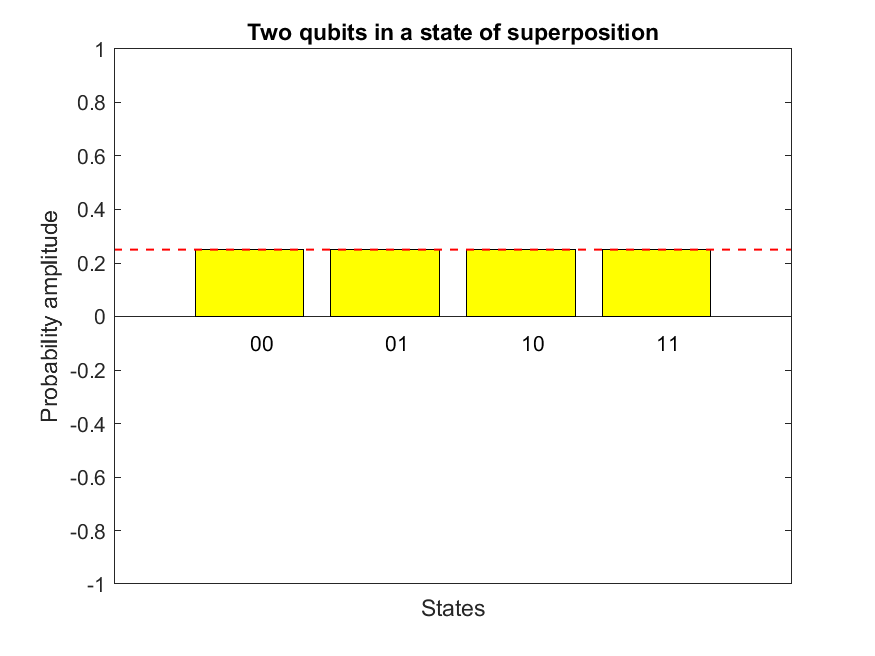
\includegraphics[width=9cm,height=9cm,keepaspectratio]{fig1.jpg}}
% 	\caption{Rectangular electrodes model.}
% 	\label{fig}
% \end{figure}



\subsection{Setup using Rectangular Electrodes}

The observation of potential and temperature changes in material for rectangular electrodes is depicted in \textbf{Figs. 2(a-d)}. The electrode gaps utilized in the setup depicted in Fig. 2 measure 100 nm. Figs.  \textbf{2(a, c)} depicts the precise state of the model at the moment of IMT occurrence, while \textbf{Figs. 2(b, d)} showcases the subsequent state following IMT and its attainment of equilibrium. Upon careful observation, it becomes evident that the material changes into a conductive state which can be observed from the changes in electric potential and temperature across the device. These results are more pronounced due to wider electrodes and more area allowing better heat transfer to substrate.Based on the provided diagram, it is evident that the IMT transition takes place precisely at a temperature of 150 K validating existing literature.

% \begin{figure}[htbp]
% 	\centerline{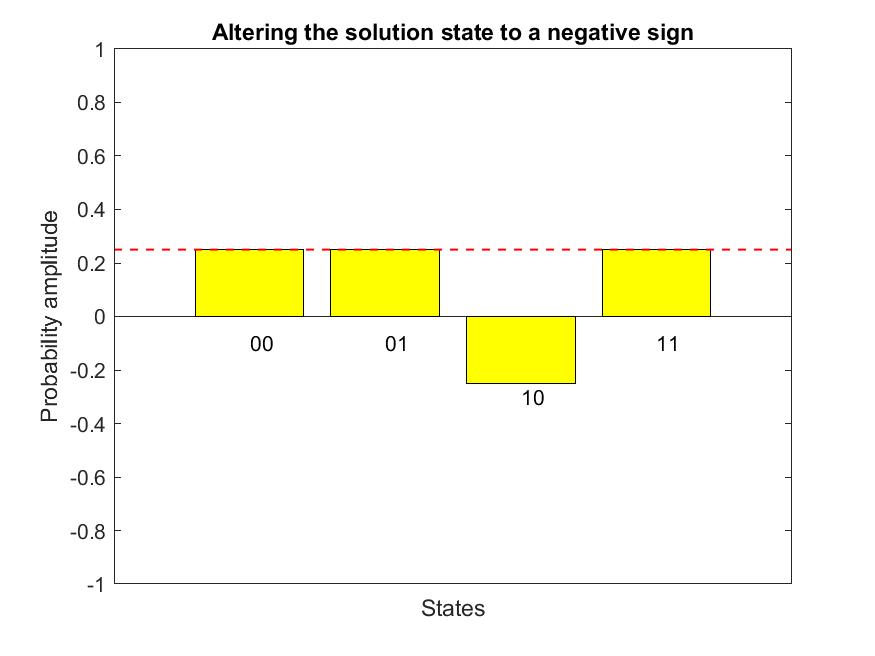
\includegraphics[width=9cm,height=10cm,keepaspectratio]{fig2.jpg}}
% 	\caption{Temperature and potential  of the 100 nm gap setup taken at different intervals for rectangular electrodes.}
% 	\label{fig}
% \end{figure}

\subsection{Setup using Triangular Electrodes}

% \begin{figure}[htbp]	\centerline{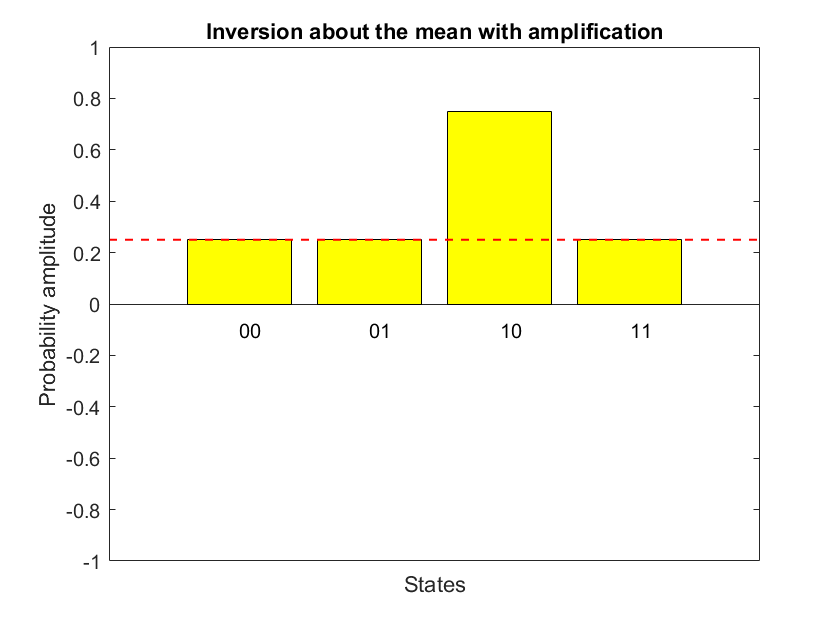
\includegraphics[width=8cm,height=8cm,keepaspectratio]{fig3.jpg}}
% 	\caption{Triangular electrodes model}
% 	\label{fig}
% \end{figure}
The potential and temperature changes in material for triangular electrodes is observed here. The geometric sharp corners of the electrodes provide the strongest electric field, as seen in \textbf{ Fig. 4}. The material's ability to resist switching is aided by the triangle electrode's ability to create strong electric fields close to the metal/oxide contact.
This characteristic enhances the material's capacity for Resistive Switching, contributing to its overall effectiveness in the process.

% \begin{figure}[htbp]
% 	\centerline{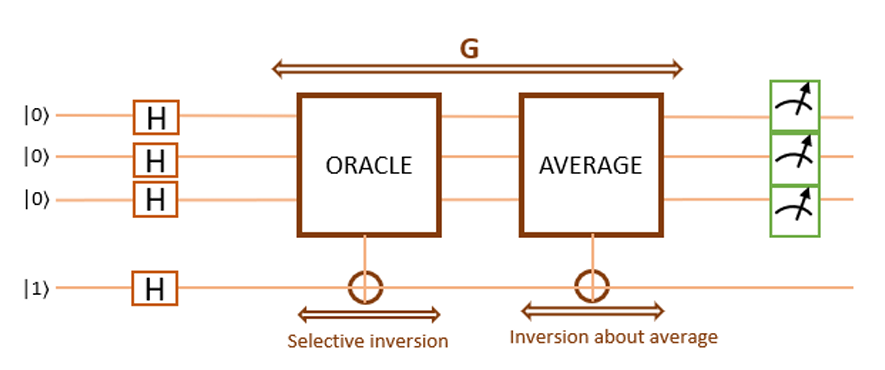
\includegraphics[width=9cm,height=10cm,keepaspectratio]{fig4.jpg}}
% 	\caption{Temperature and potential profile  of the 100 nm gap setup taken at  different intervals for triangular electrodes.}
% 	\label{fig}
% \end{figure}



\subsection{Setup using Cylindrical Electrodes}


% \begin{figure}[htbp]
% 	\centerline{\includegraphics[width=9cm,height=10cm,keepaspectratio]{fig5.jpg}}
% 	\caption{ Cylindrical electrodes model.}
% 	\label{fig}
% \end{figure}
The cylindrical electrode model differs from the previous two models in its construction. It follows a sandwiched configuration where V\textsubscript{2}O\textsubscript{3} is positioned between two electrodes, with the substrate covering the entire device.The behaviour of the setup has been depicted in \textbf{Fig 6} in which we can we clearly see the formation of conducting filament in the material V\textsubscript{2}O\textsubscript{3}. Building this setup is more expensive compared to the previous ones because those setups can take advantage of existing silicon-based fabrication methods. This particular configuration is designed primarily for academic research, as it provides complete isolation of the device through the substrate. The study focuses on observing potential and temperature changes within the material using cylindrical electrodes. In this setup, the electrode gaps are set at 100 nm, and the comparison is carried out at various intervals.These results are similar to what we observed in previous electrodes but the conducting filament is clearly observed due to the sandwiched setup.

% \begin{figure}[htbp]
% 	\centerline{\includegraphics[width=9cm,height=10cm,keepaspectratio]{fig6.jpg}}
% 	\caption{   Temperature and potential profile  of the 100 nm gap setup taken at  different intervals for Cylindrical electrodes.}
% 	\label{fig}
% \end{figure}



\subsection{Comparison of three models}

The comparison of results from all three models with a 100 nm gap aims to determine the most efficient electrode shape. Upon comparing the voltage-current (V-I) characteristics and voltage-versus-time profiles of all three models, notable insights emerge. The switching point voltage, observed at the peaks of each curve, varies among the setups. Specifically, the triangular electrode configuration exhibits the highest switching point voltage, while the rectangular setup shows the lowest. This implies that the rectangular setup boasts superior switching capabilities at lower voltages, contributing to reduced power consumption. Analyzing the resistance-versus-time curve, the triangular setup displays a significantly steeper curve, indicating faster resistance switching compared to the other models. This accelerated switching is attributed to the focusing effect inherent in the triangular configuration.



% \begin{figure}[htbp]
% 	\centerline{\includegraphics[width=8cm,height=8cm,keepaspectratio]{fig7.jpg}}
% 	\caption{Comparison of  V-I characteristics of  Rectangular, Triangular and Cylindrical electrode setups of 100 nm gap. }
% 	\label{fig}
% \end{figure}

Remarkably, the resistance switching in the rectangular electrode setup closely mirrors that of the triangular configuration. In contrast, the cylindrical setup exhibits a comparatively slower switching behavior.We evaluate resistances, V-I characteristics, and potential differences. Interestingly, the rectangular electrode outperforms the others, with lower resistance and a lower activation voltage. This superiority can be attributed to the rectangular electrode’s capacity to efficiently transfer heat to the material, thanks to its larger surface area. This outcome might appear counterintuitive, as one might expect the triangular electrode to perform better due to its focusing effect. However, the smaller contact area of the triangular electrode limits the heat transfer compared to the rectangular electrode.
% \begin{figure}[htbp]
% 	\centerline{\includegraphics[width=8cm,height=8cm,keepaspectratio]{fig8.jpg}}
% 	\caption{Comparison of resistances of  Rectangular, Triangular and Cylindrical electrode setups of 100 nm gap. }
% 	\label{fig}
% \end{figure}
% \begin{figure}[htbp]
% 	\centerline{\includegraphics[width=8cm,height=8cm,keepaspectratio]{fig9.jpg}}
% 	\caption{Comparison of Potential differences of  Rectangular, Triangular and Cylindrical electrode setups of 100 nm gap.
% 	 }
% 	\label{fig}
% \end{figure}
The cylindrical electrode exhibits the least favorable performance, primarily due to the difficulty in achieving higher temperatures in this configuration, owing to the larger substrate. This underscores the importance of prioritizing heat accumulation when designing these setups. Furthermore, this observation supports the validity of the Joule heating model in understanding the Insulator-to-Metal Transition (IMT) in Mott devices

\section{Conclusion}
This study thoroughly investigated and modeled the Mott insulator V\textsubscript{2}O\textsubscript{3}, exploring its potential for ReRAM technology. The impact of various electrode configurations on device performance was carefully examined, identifying crucial areas for improvement crucial for successful integration. These results are pivotal for advancing the use of Mott materials in emerging memory technologies. The insights gained from this research are particularly valuable for developing a practical, physical model for future applications.




\begin{thebibliography}{00}

	\bibitem{b1} T. N. Theis and P. M. Solomon, "In Quest of the “Next Switch”: Prospects for Greatly Reduced Power Dissipation in a Successor to the Silicon Field-Effect Transistor," in Proceedings of the IEEE, vol. 98, no. 12, pp. 2005-2014, Dec. 2010.

	\bibitem{b2} Molas, G.; Nowak, E. "Advances in Emerging Memory Technologies: From Data Storage to Artificial Intelligence," Appl. Sci., vol. 11, no. 23, p. 1254, 2021.

	\bibitem{b3} J. H. de Boer, and E. J. W Verwey, "Semi-conductors with partially and with completely filled 3d-lattice bands," Proceedings of the Physical Society, vol. 49 (4S), pp. 4S, Aug.1937.

	\bibitem{b4} E. Janod, J. Tranchant, B. Corraze, M. Querré, P. Stoliar, M. Rozenberg, T. Cren et al. "Resistive switching in Mott insulators and correlated systems," Advanced Functional Materials, vol. 25, no. 40, pp. 6287-6305, Oct.2015.

	\bibitem{b5} J. Hubbard, "Electron correlations in narrow energy bands. II. The degenerate band case." Proceedings of the Royal Society of London. Series A. Mathematical and Physical Sciences, vol. 277, no. 1369, pp. 237-259, Jan.1964.

	\bibitem{b6} C. N. Berglund, "Thermal filaments in vanadium dioxide," in IEEE Transactions on Electron Devices, vol. 16, no. 5, pp. 432-437, May 1969.

	\bibitem{b7} A. Ronchi et al., "Light-Assisted Resistance Collapse in a V\textsubscript{2}O\textsubscript{3}-Based Mott-Insulator Device," Phys. Rev. Appl., vol. 15, no. 4, pp. 044023, Apr. 2021.

	\bibitem{b8} V. N. Andreev et al., "Thermal conductivity of VO\textsubscript{2}, V3O5, and V\textsubscript{2}O\textsubscript{3}," physica status solidi (a), vol. 48, no. 2, pp. K153-K156, 1978.

	\bibitem{b9} P. Stoliar et al., "Universal electric-field-driven resistive transition in narrow-gap Mott insulators," Adv. Mater., vol. 25, pp. 3222, 2013.

	\bibitem{b10} S. Guénon et al., "Electrical breakdown in a V\textsubscript{2}O\textsubscript{3} device at the insulator-to-metal transition," EPL (Europhysics Letters), vol. 101, pp. 57003, 2013.

	\bibitem{b11} P. Homm et al., "Collapse of the low temperature insulating state in Cr-doped V\textsubscript{2}O\textsubscript{3} thin films," Appl. Phys. Lett., vol. 107, pp. 111904, 2015.

	\bibitem{b12} Y. Kalcheim et al., "Non-thermal resistive switching in Mott insulator nanowires," Nat. Commun., vol. 11, pp. 2985, 2020.

	\bibitem{b13} M. M. Qazilbash et al., "Electrodynamics of the vanadium oxides VO\textsubscript{2} and V\textsubscript{2}O\textsubscript{3}," Phys. Rev. B, vol. 77, pp. 115121, 2008.

	\bibitem{b14} P. Paweł, J. Jamroz, and T. K. Pietrzak, “Observation of metal–insulator transition (mit) in vanadium oxides V\textsubscript{2}O\textsubscript{3} and VO\textsubscript{2} in xrd, dsc and dc experiments,” Crystals, 2023.

	\bibitem{b15} P. Homm, M. Menghini, J. W. Seo, S. Peters, and J. P. Locquet, “Room temperature Mott metal–insulator transition in V\textsubscript{2}O\textsubscript{3} compounds induced via strain-engineering,” APL Materials, vol. 9, no. 2, pp. 021116, Feb  2021.

	\bibitem{b16} F. Mazzola, S. K. Chaluvadi, V. Polewczyk, D. Mondal, J. Fujii, P. Rajak, M. Islam, R. Ciancio, L. Barba, M. Fabrizio, G. Rossi, P. Orgiani, and I. Vobornik, “Disentangling structural and electronic properties in V\textsubscript{2}O\textsubscript{3} thin films: A genuine non symmetry breaking mott transition,” Nano Letters, vol. 22, no. 14, pp. 5990–5996, 2022.

	\bibitem{b17} H. Kizuka et al., “Temperature dependence of thermal conductivity of VO\textsubscript{2} thin films across metal–insulator transition,” Japanese Journal of Applied Physics, vol. 98, no. 053201, 2015.

	\bibitem{b18} H. Y. Peng, L. Pu, J. C. Wu, D. Cha, J. H. Hong, W. N. Lin, Y. Y. Li, J. F. Ding, A. David, K. Li, and T. Wu, “Effects of electrode material and configuration on the characteristics of planar resistive switching devices,” APL Materials, vol. 1, no. 5, pp. 052106, Nov  2013.
\end{thebibliography}

\end{document}
